\documentclass[../../../../main.tex]{subfiles}
\begin{document}

\begin{flushright}
\footnotesize\textit{【自動文字起こし・要確認】}
\end{flushright}

\noindent
\textbf{[解1]} $f(x) = \dfrac{x^2(2 \cdot 3^3 \cdot n - x)}{2^5 \cdot 3^2 \cdot n^2}$ において, $k \in \mathbb{Z}$ として,
\[
\begin{cases}
|f(k+1) - f(k)| \le 1 \text{ なら, } [f(k+1)] = [f(k)], [f(k)] \pm 1 \\
|f(k+1) - f(k)| \ge 1 \text{ なら, } [f(k+1)] \neq [f(k)]
\end{cases}
\quad \dots \text{＊}
\]
である.
\begin{align*}
f(k+1) - f(k) &= \frac{1}{2^5 \cdot 3^2 \cdot n^2} \left[ (k+1)^2(2 \cdot 3^3 \cdot n - k - 1) - k^2(2 \cdot 3^3 \cdot n - k) \right] \\
&= \frac{1}{2^5 \cdot 3^2 \cdot n^2} \left[ (2k+1)(2 \cdot 3^3 \cdot n - k) - (k+1)^2 \right] \\
&= \frac{1}{2^5 \cdot 3^2 \cdot n^2} \left[ -3k^2 + (2 \cdot 3^3 \cdot n - 3)k + 2 \cdot 3^3 \cdot n - 1 \right] \quad \dots \text{①}
\end{align*}
ここで, $2^5 \cdot 3^2 \cdot n^2 \cdot f'(x) = 3x(2^2 \cdot 3^2 \cdot n - x)$ から, $0 \le x \le 36n$ では $f'(x) \ge 0$ となり, $f(x)$ は単調増加である. $g(k) = f(k+1) - f(k) - 1$ とおくと, ①から,
\[
2^5 \cdot 3^2 \cdot n^2 g(k) = -3k^2 + 3(2^2 \cdot 3^2 \cdot n - 1)k + 2 \cdot 3^3 \cdot n - 1 - 2^5 \cdot 3^2 \cdot n^2
\]
なので, $g(k) = 0$ の解は,
\begin{align*}
k &= \frac{1}{6} \left[ 3(2^2 \cdot 3^2 \cdot n - 1) \pm \sqrt{9(2^2 \cdot 3^2 \cdot n - 1)^2 - 12\left(2^5 \cdot 3^2 \cdot n^2 + 1 - 2 \cdot 3^3 \cdot n\right)} \right] \\
&= \frac{1}{6} \left[ 3(2^2 \cdot 3^2 \cdot n - 1) \pm \sqrt{2^4 \cdot 3^4 \cdot n^2 - 3} \right] \quad \dots \text{②}
\end{align*}
ここで $2^2 \cdot 3^2 \cdot n - 3 < \sqrt{2^4 \cdot 3^4 \cdot n^2 - 3} < 2^2 \cdot 3^2 \cdot n$ だから, $0 \le k$ の範囲で $g(k) \ge 0$ となる $k \in \mathbb{Z}$ は, ②から,
\[
12n \le k \le 24n - 1 \quad \dots \text{③}
\]
である. $f(x)$ の単調性および ＊ から,
\[
\begin{cases}
k = 0, 1, \dots, 12n-1 \text{ の時, } [f(k+1)] = [f(k)], [f(k)] + 1 \\
k = 12n, \dots, 24n-1 \text{ の時, } [f(k+1)] > [f(k)] \\
k = 24n, \dots, 36n \text{ の時, } [f(k+1)] = [f(k)], [f(k)] + 1
\end{cases}
\]
だから,
\[
[f(0)] \le [f(1)] \le \dots \le [f(12n)] < [f(12n+1)] < \dots < [f(24n)] \le \dots \le [f(36n)]
\]
となり,
\[
[f(0)] = 0, \quad [f(12n)] = 7n, \quad [f(24n)] = 20n, \quad [f(36n)] = 27n
\]
だから求めるのは
\[
(7n + 1) + (24n - 1 - 12n) + (27n + 1 - 20n) = 26n + 1 \text{ 個}
\]

\begin{center}
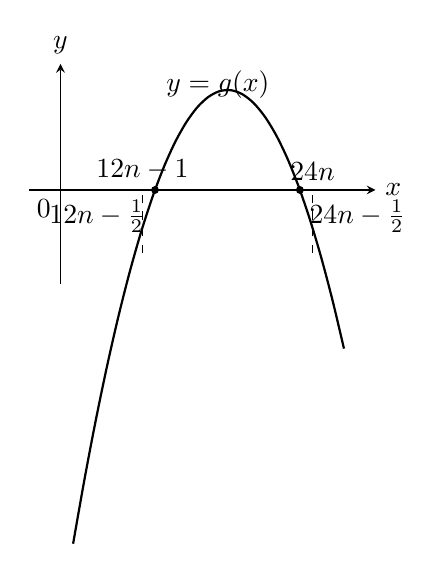
\begin{tikzpicture}[scale=0.8, >=stealth]
\draw[->] (-0.5,0) -- (5,0) node[right] {$x$};
\draw[->] (0,-1.5) -- (0,2) node[above] {$y$};
\draw[domain=0.2:4.5, smooth, variable=\x, thick] plot ({\x}, {-1.2*(\x-1.5)*(\x-3.8)});
\node[above] at (2.5, 1.3) {$y = g(x)$};
\filldraw (1.5,0) circle (1.5pt) node[below left] {$12n - \frac{1}{2}$};
\filldraw (3.8,0) circle (1.5pt) node[below right] {$24n - \frac{1}{2}$};
\draw[dashed] (1.3, -1) -- (1.3, 0) node[above] {$12n-1$};
\draw[dashed] (4.0, -1) -- (4.0, 0) node[above] {$24n$};
\node[below left] at (0,0) {$0$};
\end{tikzpicture}
\end{center}

\bigskip

\noindent
\textbf{[解2]} (以下) 平均値の定理から,
\[
f(k+1) - f(k) = f'(a_k) \quad (k < a_k < k+1) \quad \dots \text{①'}
\]
を満たす $a_k$ がある.
\[
f'(x) = \frac{x(2^2 \cdot 3^2 \cdot n - x)}{2^5 \cdot 3^2 \cdot n^2} \le 1 \iff -x^2 + 2^2 \cdot 3^2 \cdot n \cdot x - 2^5 \cdot 3^2 \cdot n^2 \le 0 \iff x \le 12n, 24n \le x
\]
だから, ①'とあわせて
\[
\begin{cases}
k = 0, 1, \dots, 12n-1 \text{ の時, } f(k+1) - f(k) < 1 \\
k = 12n, 12n+1, \dots, 24n-1 \text{ の時, } f(k+1) - f(k) > 1 \\
k = 24n, 24n+1, \dots, 36n \text{ の時, } f(k+1) - f(k) < 1
\end{cases}
\]
となって[解1]の③に帰着する.

\newpage

\end{document}
